\documentclass[tikz,border=10pt]{standalone}
% Parallelogram BADC with point E on AD; scale s = 0.014235 cm/px (from STYLE METRICS)
\begin{document}
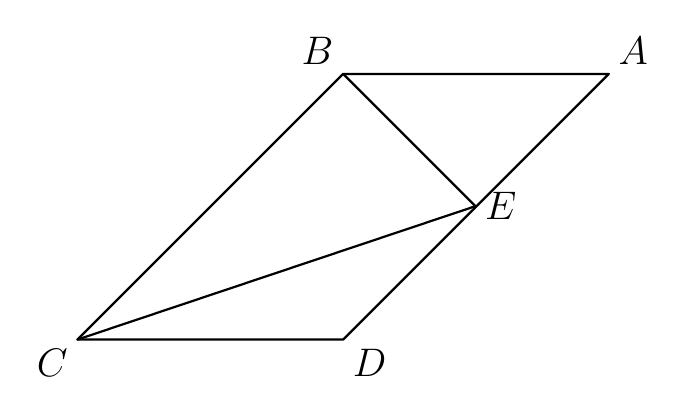
\begin{tikzpicture}[line join=round, line cap=round]
  % Vertices (TikZ cm), origin at image centre (305,182) with y flipped
  \coordinate (B) at (0,1.680);
  \coordinate (A) at (3.374,1.680);
  \coordinate (D) at (0,-1.694);
  \coordinate (C) at (-3.374,-1.694);
  \coordinate (E) at (1.680,0);

  % Parallelogram sides BA, AD, DC, CB
  \draw[solid, black, line width=0.8pt] (B) -- (A) -- (D) -- (C) -- cycle;

  % Interior segments BE and CE
  \draw[solid, black, line width=0.8pt] (B) -- (E);
  \draw[solid, black, line width=0.8pt] (C) -- (E);

  % Labels (15pt font from cap-height metric)
  \node[above left]  at (B) {\fontsize{15}{18}\selectfont $B$};
  \node[above right] at (A) {\fontsize{15}{18}\selectfont $A$};
  \node[below right] at (D) {\fontsize{15}{18}\selectfont $D$};
  \node[below left]  at (C) {\fontsize{15}{18}\selectfont $C$};
  \node[right]       at (E) {\fontsize{15}{18}\selectfont $E$};
\end{tikzpicture}
\end{document}